\labeledsection{Statistical Learning}{sec:statistical_learning}
\anondefinition{
\defemph{Statistical Learning} has the goal to learn the correct \linkterm{probability distribution}{def:prob_distribution} of a \linkterm{random variable}{def:random_variable}
}{statistical_learning}

\Example{
\begin{itemize}
    \item Bayesian learning: learning probabilistic models (e.g. the \linkterm{CPD}{def:cond_prob_distribution} in \linkterm{Bayesian Networks}{def:bayes_net}) from observations.
    \item Maximum a Posteriori and Maximum Likelihood Learning
    \item \linkterm{Bayesian Networks}{def:bayes_net} Learning
\end{itemize}
}{}

\redbox{
We will discuss these topics but let's first explain the running example:
}

\Example{
\begin{figure}[H]
    \centering
    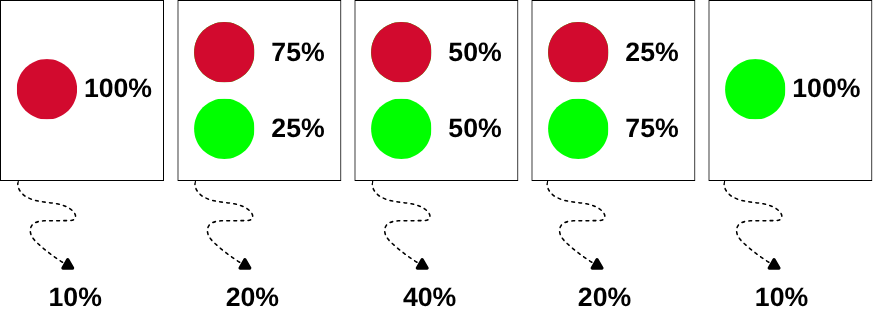
\includegraphics[width=0.6\linewidth]{images/candies.png}
\end{figure}

We have two flavors of candies, cherry and lime. We have five kinds of bags of candies where each kind contains different numbers of both flavors. 

We know that $10\%$ of our boxes contain only cherry candies, etc. We express that as \linkterm{priors}{def:bayesian_terms} of five \linkterm{hypotheses}{supervised_learning} $h_1 = 0.1, h_2=0.3, \cdots h_5 = 0.1$

We observed $10$ lime candies  drawn from some bag (which we do not know), we want to know what kind of bag it is and what flavor will the next candy be?

\textbf{Note: }every \linkterm{hypothesis}{supervised_learning} $h_i$ is itself a \linkterm{probability distribution}{def:prob_distribution} over the \linkterm{random variable}{def:random_variable} \textit{flavor}
}{candies_example}

Let $d_i$ be the event that the $i-$th drawn candy is green (lime), then the \linkterm{posterior}{def:bayesian_terms} of the \linkterm{hypotheses}{supervised_learning} keeps updating as $n$ increases for lime observations $\mathbf{d} =  d_{1:n}$:

\begin{figure}[H]
    \centering
    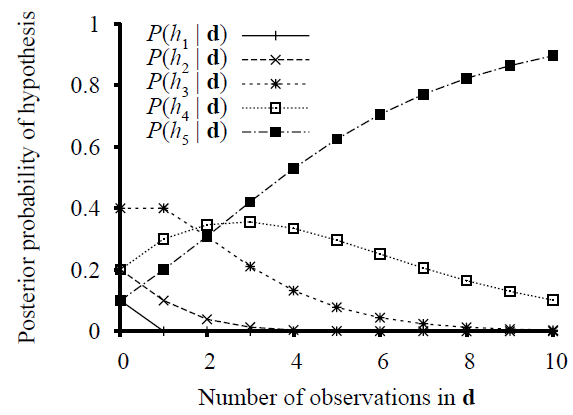
\includegraphics[width=0.6\linewidth]{images/candies_post.png}
\end{figure}

If the observations are \linkterm{IID}{def:iid}:
\[
P(d \mid h_i) = \prod_{j} P(d_j \mid h_i)
\]

\titledbox{Remember}{
\linkterm{likelihood}{def:bayesian_terms} $P(B \mid A)$ is the probability that the evidence $B$ would be observed if the hypothesis $A$ were true. (\Defref{def:bayesian_terms})
}

The \linkterm{likelihood}{def:bayesian_terms} of our observation $\mathbf{d} = d_{1:10}$ (10 lime candies) under each hypothesis $h_i$ is calculated as:
\begin{align*}
P(\mathbf{d} \mid h_1) &= (0.0)^{10} = 0 \\ 
P(\mathbf{d} \mid h_2) &= (0.25)^{10} = \frac{1}{1,048,576} \approx 9.54 \times 10^{-7} \\
P(\mathbf{d} \mid h_3) &= (0.5)^{10} = \frac{1}{1,024} \approx 9.77 \times 10^{-4} \\ 
P(\mathbf{d} \mid h_4) &= (0.75)^{10} = \frac{59,049}{1,048,576} \approx 0.0563 \\
P(\mathbf{d} \mid h_5) &= (1.0)^{10} = 1 
\end{align*}


The \linkterm{posterior}{def:bayesian_terms} probabilities originate from the hypothesis \linkterm{priors}{def:bayesian_terms} and are dynamically updated as data is observed.

\questionbox{
What is the probability that the $n+1$ candy is lime? 
}

\answerbox{
We compute the \linkterm{expected value}{expected_value} of the probability of the next candy being lime over all \linkterm{hypotheses}{supervised_learning}
\begin{align*}
P(d_{n+1} = \text{lime} \mid \mathbf{d}) 
&= \sum_{i} P(d_{n+1} = \text{lime} \land h_i \mid \mathbf{d}) \\
&= \sum_{i} \frac{P(d_{n+1} = \text{lime} \land h_i \land \mathbf{d})}{P(\mathbf{d})} \\
&= \sum_{i} \frac{P(d_{n+1} = \text{lime} \mid h_i, \mathbf{d}) \cdot P(h_i \land \mathbf{d})}{P(\mathbf{d})} \\
&= \sum_{i} P(d_{n+1} = \text{lime} \mid h_i, \mathbf{d}) \cdot \frac{P(h_i \land \mathbf{d})}{P(\mathbf{d})} \\
&= \sum_{i} P(d_{n+1} = \text{lime} \mid h_i, \mathbf{d}) \cdot P(h_i \mid \mathbf{d}) \\
&= \sum_{i} P(d_{n+1} = \text{lime} \mid h_i) \cdot P(h_i \mid \mathbf{d}) 
\end{align*}
}

We obtain the following predictions for different numbers of observed limes:
\begin{figure}[H]
    \centering
    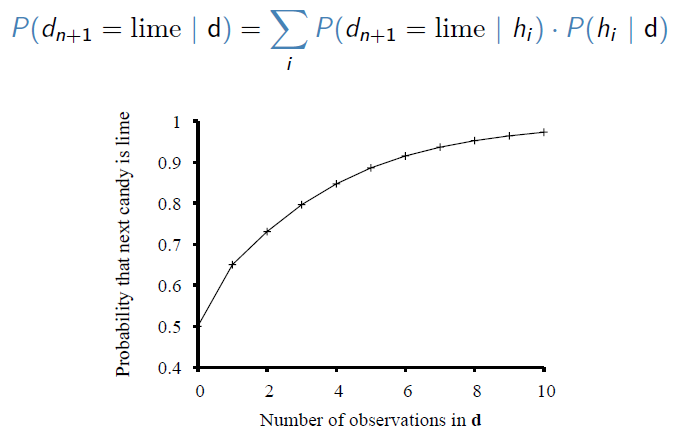
\includegraphics[width=0.6\linewidth]{images/candies_predictions.png}
\end{figure}

\anondefinition{
\defemph{Bayesian Learning} calculates the probability of each \linkterm{hypothesis}{supervised_learning} and makes predictions based on this
\begin{itemize}
    \item Given the data so far, each \linkterm{hypothesis}{supervised_learning} has a \linkterm{posterior}{def:bayesian_terms} probability:
    \[
        P(h_i \mid d) = \alpha (P(d \mid h_i) \cdot P(h_i))    
    \]
    where $P(d \mid h_i)$ is called the \linkterm{likelihood}{def:bayesian_terms} of the data under $h_i$ and $P(h_i)$ the \linkterm{hypothesis}{supervised_learning} \linkterm{prior}{def:bayesian_terms}
    \item \defemph{Bayesian Predictions} uses a \linkterm{likelihood}{def:bayesian_terms}-weighted average over the \linkterm{hypotheses}{supervised_learning}:
    \[
    \probd{X \mid d} := \sum_{i} \probd{X \mid h_i} \cdot P(h_i \mid d)
    \]
\end{itemize}
}{Bayesian_Learning}



\problembox{
Summing over the \linkterm{hypothesis space}{supervised_learning} is often interactable
}

\solutionbox{
Approximate the learning methods to simplify
}

\ideabox{
Make predictions w.r.t the \textit{"most probable"} \linkterm{hypothesis}{supervised_learning}
}

\anondefinition{
We call a \linkterm{hypothesis}{supervised_learning} $h_i$ that maximizes $P(h_i \mid d)$ a \defemph{Maximum a Posteriori (MAP) hypothesis} and refer to it as $h_{\text{MAP}}$
}{MAP_hyp}

\anondefinition{
\defemph{Maximum a Posteriori (MAP) Learning} chooses the \linkterm{MAP Hypthesis}{MAP_hyp}
}{MAP_learning}

\observationbox{
Predictions made according to a \linkterm{MAP hypothesis $h_{\text{MAP}}$}{MAP_hyp} are approximately \linkterm{Bayesian}{Bayesian_Learning} to the extent that $\probd{X \mid d} \approx \probd{X \mid h_{\text{MAP}}}$
}

\Example{
In our candy example, \linkterm{$h_{\text{MAP}}$}{MAP_hyp} = 5 after three limes in a row 
\begin{itemize}
    \item a \linkterm{MAP learner}{MAP_learning} would predict that candy $4$ is lime with probability of $1$
    \item \linkterm{Full Bayesian Learning}{Bayesian_Learning} would predict that of $0.8$ (see prediction curve)
\end{itemize}
}{}

\commandnote{
As more data arrive, the \linkterm{MAP}{MAP_learning} and \linkterm{Bayesian}{Bayesian_Learning} predictions become closer, because the competitors to the \linkterm{MAP hypothesis $h_{\text{MAP}}$}{MAP_hyp} become less and less probable.
}

\redbox{
Finding \linkterm{MAP hypotheses}{MAP_hyp} is often much easier than \linkterm{Bayesian Learning}{Bayesian_Learning}, because it requires solving an optimization problem instead of a large summation (or integration) problem
}

\titledbox{$\log$ Trick}{
Maximizing $P(h_i \mid d)$ means maximizing the product $P(d \mid h_i) \cdot P(h_i)$. To maximize that, we can maximize 
\[
\log_2 (P(d \mid h_i) \cdot P(h_i))
\]


$\leadsto$ maximizing the summation $\log_2 P(d \mid h_i) + \log_2 P(h_i)$
}

\titledbox{Minimization Trick}{
Instead of maximizing $\log_2 P(d \mid h_i) + \log_2 P(h_i)$ we can minimize:
\[
- \log_2 P(d \mid h_i) - \log_2 P(h_i)
\]
}

\anondefinition{
Let $x$ be a specific outcome of a \linkterm{random variable}{def:random_variable} $X$ with probability $P(X=x)$. The \defemph{self-information} (also called \defemph{information content} or \defemph{Shannon information}) of $x$ is:
\[
I(x) := -\log_2(P(x))
\]
}{self_information}

\titledbox{Sounds familiar?}{
The relationship between \linkterm{individual self-information}{self_information} $I(x)$ and the  \linkterm{total entropy}{entropy} $I(\tuple{p_1, \cdots, p_n})$ of a \linkterm{probability distribution}{def:prob_distribution} is that \linkterm{entropy}{entropy} is the \linkterm{expected value}{expected_value} (weighted average) of the \linkterm{self-information}{self_information} across all possible outcomes.

If we substitute the \linkterm{self-information}{self_information} of a single outcome, $I(x_i) = -\log_2(p_i)$, into the definition of \linkterm{entropy}{entropy}, we see this connection directly:

\[
I(\tuple{p_1, \cdots, p_n}) = \sum_{i=1}^{n} p_i \cdot \underbrace{\left(-\log_2(p_i)\right)}_{\text{Self-Information } I(x_i)} = \mathbb{E}[I(X)]
\]
}


\titledbox{Intuition}{
\begin{itemize}
    \item If an event $x$ is almost certain to happen ($P(x) \approx 1$), seeing it occur tells us practically nothing new. Its \textit{surprisal} is close to $0$.
    \item If an event is incredibly rare ($P(x) \approx 0$), its occurrence is a massive shock. It carries a high amount of new information, so its \textit{surprisal} is very large.
\end{itemize}

While \linkterm{entropy}{entropy} measures the \textit{average} uncertainty of an entire system, \linkterm{self-information}{self_information} measures the exact amount of \textit{"surprise"} packed into a \textit{single, specific} outcome.
}

\questionbox{
How do we turn this abstract concept of \textit{"surprise"} into something measurable, like \linkterm{bits}{bit_info}?
}

\ideabox{
Imagine a communication game where I need to transmit an outcome $x$ to someone over a network using a binary code (\texttt{0}s and \texttt{1}s).
To make the transmission as efficient as possible, I should use a clever strategy:
\begin{itemize}
    \item \textbf{Frequent outcomes} (low self-information / low surprise) should get very short codes (e.g., just a single bit like \texttt{0}) because they are sent constantly.
    \item \textbf{Rare outcomes} (high self-information / high surprise) can be given much longer codes (e.g., \texttt{11010}) because we rarely have to send them.
\end{itemize}
}

\titledbox{Shannon's source coding theorem}{
The absolute shortest binary code length possible to represent an outcome $x$ without losing data is exactly equal to its \linkterm{self-information}{self_information}, $-\log_2 P(x)$. This gives our abstract mathematical surprise a physical, practical meaning: it is the number of bits needed to write the outcome down.
}

\anondefinition{
The \defemph{Description Length} $L(x)$ of an outcome $x$ is the optimal number of bits required to uniquely encode and transmit $x$ under a \linkterm{probability distribution}{def:prob_distribution} $\probd{X}$. It is defined as:
\[
L(x) := I(x) = -\log_2 P(x)
\]
}{description_length}

\questionbox{
What minimizing $- \log_2 P(d \mid h_i) - \log_2 P(h_i)$ means?
}

\answerbox{
\begin{itemize}
    \item $- \log_2 P(\mathbf{d} \mid h_i) = L(\mathbf{d} \mid h_i)$ is the \linkterm{description length}{description_length} of the data given the \linkterm{hypothesis}{supervised_learning}:
    This is the number of \linkterm{bits}{bit_info} needed to encode the observed data $\mathbf{d}$ when using the hypothesis $h_i$ as our \textit{"compression guide"}. 
    \begin{itemize}
        \item If $h_i$ predicts the data perfectly ($P=1$), this term becomes $0$ bits—the data is entirely expected and costs nothing extra to record.
        \item If the data contains anomalies, noise, or deviations that contradict $h_i$, we must expend extra \linkterm{bits}{bit_info} to specify these unpredicted details. Minimizing this term forces us to find an \textbf{accurate model} that fits the observations tightly.
    \end{itemize}
    
    \item $- \log_2 P(h_i) = L(h_i)$ is the \linkterm{description length}{description_length} of the \linkterm{hypothesis}{supervised_learning}:
    This is the number of \linkterm{bits}{bit_info} needed to specify the parameters or structure of the \linkterm{hypothesis}{supervised_learning} $h_i$ itself before seeing any data.
    \begin{itemize}
        \item A simple, generic \linkterm{hypothesis}{supervised_learning} has a high \linkterm{prior probability}{def:bayesian_terms}, meaning it is concise and cheap to write down (low \linkterm{description length}{description_length}).
        \item A highly complex hypothesis has a low \linkterm{prior probability}{def:bayesian_terms}, meaning it requires many \linkterm{bits}{bit_info} to fully specify. Minimizing this term forces us to prefer \textbf{simpler models}.
    \end{itemize}
\end{itemize}

\textbf{Conclusion:} Minimizing their sum means finding a \linkterm{hypothesis}{supervised_learning} $h_i$ that achieves the perfect transmission trade-off. We want a model that is compact to state ($L(h_i)$ is small), but accurate enough that it doesn't leave behind a massive, costly trail of unpredicted data corrections ($L(\mathbf{d} \mid h_i)$ is small).
}

\anondefinition{
We call a \linkterm{hypothesis}{supervised_learning} $h_i$ that minimizes the combined total \linkterm{description length}{description_length} of both the model itself and the data given that model the \defemph{Minimum Description Length (MDL) hypothesis} and refer to it as $h_{\text{MDL}}$
}{MDL_hyp}

\anondefinition{
\defemph{Minimum Description Length (MDL) Learning} chooses the \linkterm{MDL hypothesis $h_{\text{MDL}}$}{MDL_hyp} by solving the optimization problem:
\[
h_{\text{MDL}} = \arg\min_{h_i} \Big( L(h_i) + L(\mathbf{d} \mid h_i) \Big)
\]
}{MDL_learning}

\observationbox{
The MDL principle provides a strict, information-theoretic formulation of \textbf{Occam's Razor}.
}



\problembox{
What if we have no prior reason to prefer one hypothesis over another?
}

\ideabox{
Assume a \textbf{uniform prior distribution}: every hypothesis in our hypothesis space is equally likely, meaning $P(h_1) = P(h_2) = \cdots = P(h_n)$. 

In terms of communication and description lengths, this means every hypothesis requires the exact same number of bits to describe ($L(h_i) = \text{constant}$ for all $i$).
}

\titledbox{Dropping the Constant}{
If we look back at our \linkterm{MDL optimization problem}{MDL_learning}, a constant model length changes our objective dramatically:
\[
h = \arg\min_{h_i} \Big( \underbrace{L(h_i)}_{\text{constant}} + L(\mathbf{d} \mid h_i) \Big) \implies h = \arg\min_{h_i} L(\mathbf{d} \mid h_i)
\]

Minimizing the \linkterm{description length}{description_length} $L(\mathbf{d} \mid h_i)$ is identical to maximizing the \linkterm{likelihood}{def:bayesian_terms} $P(\mathbf{d} \mid h_i)$. 

When we completely ignore the prior probabilities of the models and focus entirely on how well a model explains the data, we enter the realm of \defemph{Maximum Likelihood Learning}.
}

\anondefinition{
We call a \linkterm{hypothesis}{supervised_learning} $h_i$ that maximizes the \linkterm{likelihood}{def:bayesian_terms} of the observed data $P(\mathbf{d} \mid h_i)$ a \defemph{Maximum Likelihood (ML) hypothesis} and refer to it as $h_{\text{ML}}$
}{ML_hyp}

\anondefinition{
\defemph{Maximum Likelihood (ML) Learning} chooses the \linkterm{ML Hypothesis}{ML_hyp} by maximizing the data likelihood directly:
\[
h_{\text{ML}} = \arg\max_{h_i} P(\mathbf{d} \mid h_i)
\]
}{ML_learning}

\Example{
Let's look back at our candy bag observations ($\mathbf{d} = 10 \text{ lime candies}$). 
\begin{itemize}
    \item A \linkterm{MAP learner}{MAP_learning} or \linkterm{MDL learner}{MDL_learning} factors in the fact that bag $h_5$ is rare ($P(h_5) = 0.1$) compared to bag $h_4$ ($P(h_4) = 0.4$), balancing simplicity/priors against the data.
    \item An \linkterm{ML learner}{ML_learning} ignores those initial bag proportions entirely. It simply asks: \textit{"Under which bag description is getting 10 limes in a row the least surprising?"} Since $P(\mathbf{d} \mid h_5) = 1.0^{10} = 1$, it immediately picks $h_{\text{ML}} = h_5$.
\end{itemize}
}{}


\problembox{
\linkterm{Bayesian Networks}{def:bayes_net} often feature nodes with a particular \linkterm{parametric distribution}{parametric_def} $D(\theta)$ (e.g. \linkterm{normal}{normal_dist}, \linkterm{binomial}{binomial_dist}, \linkterm{Poisson}{poisson_dist}, etc.). 
}

\titledbox{Shifting to a Continuous Continuum of Hypotheses}{
In our previous candy bag example, our hypothesis space was discrete and finite, consisting of exactly five distinct hypotheses: $\mathcal{H} = \{h_1, h_2, h_3, h_4, h_5\}$. 

But now, suppose we get a candy bag from a brand-new manufacturer, and we have absolutely no prior knowledge about the bag's contents. The true fraction of cherry candies could be any real number between $0$ and $1$. 

This means we are now searching through a continuous, infinite continuum of candidate hypotheses, where each individual hypothesis is indexed by a parameter $\theta \in [0, 1]$:
\[
h_{\theta} := \text{The hypothesis that the true probability of drawing a cherry candy is } \theta
\]
}

\Example{
Let's represent this new manufacturer scenario as a single-node Bayesian network:

\begin{figure}[H]
    \centering
    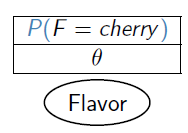
\includegraphics[width=0.15\linewidth]{images/flavor_bn.png}
\end{figure}

Every specific value of $\theta$ defines a unique candidate hypothesis $h_{\theta}$. Just like our discrete hypotheses from before, every single continuous hypothesis $h_{\theta}$ is itself a valid \linkterm{probability distribution}{def:prob_distribution} over the \linkterm{random variable}{def:random_variable} \textit{flavor}.
}{continuous_candy_example}

\commandnote{
Since we are dealing with a discrete \linkterm{random variable}{def:random_variable} \textit{flavor}, our hypothesis $h_{\theta}$ sets the probability of a specific outcome directly as its parameter: $P(\text{Flavor} = \text{cherry} \mid h_{\theta}) = \theta$. This is somewhat boring, but simple.
}

\questionbox{
How do we calculate the \linkterm{likelihood}{def:bayesian_terms} of our data $\mathbf{d}$ under a specific continuous hypothesis $h_{\theta}$?
}

\answerbox{
Let our data $\mathbf{d} = d_{1:N}$ be a specific recorded sequence of $N$ draws containing a total of $c$ cherry candies and $l$ lime candies (where $c + l = N$). 

Because the observations are \linkterm{IID}{def:iid}, the probability of observing this exact sequence under the hypothesis $h_{\theta}$ follows the exact same sequential product rule we used for our discrete hypotheses:

\[
P(\mathbf{d} \mid h_{\theta}) = \prod_{j=1}^{N} P(d_j \mid h_{\theta})
\]

According to the definition of our hypothesis $h_{\theta}$, each observed cherry candy has a probability of $\theta$, and each observed lime candy has a probability of $(1-\theta)$. Multiplying these individual probabilities across our sequence yields:
\[
P(\mathbf{d} \mid h_{\theta}) = \theta^c (1-\theta)^l
\]
}

\commandnote{
Notice how cleanly this keeps the original structure. Because our dataset $\mathbf{d} = d_{1:N}$ is an ordered sequence of actual events, the likelihood of the data given the hypothesis $h_{\theta}$ is purely the product of those outcomes, $\theta^c (1-\theta)^l$. No binomial coefficients are needed, and the hypothesis $h_{\theta}$ remains the central focus of the calculation.
}


\anondefinition{
We call a continuous hypothesis $h_{\theta}$ that maximizes the data likelihood $P(\mathbf{d} \mid h_{\theta})$ a \defemph{Maximum Likelihood Parameter (MLP) hypothesis} and refer to it as $\theta_{\text{ML}}$
}{MLP_hyp}

\anondefinition{
\defemph{Maximum Likelihood Parameter (MLP) Learning} finds the optimal parameter vector $\theta_{\text{ML}}$ by maximizing the likelihood of the observed sequence directly:
\[
\theta_{\text{ML}} = \arg\max_{\theta} P(\mathbf{d} \mid h_{\theta})
\]
}{MLP_learning}

\observationbox{
\[
\theta_{\text{ML}} = \arg\max_{\theta} \prod_{j=1}^{N} P(d_j \mid h_{\theta})
\]
}


\titledbox{Log Trick}{
To avoid maximizing a giant product, instead of maximizing $P(\mathbf{d} \mid h_{\theta})$, we maximize $\log_2 P(\mathbf{d} \mid h_{\theta})$

\begin{align*}
\theta_{\text{ML}} &= \arg\max_{\theta} P(\mathbf{d} \mid h_{\theta}) \\ 
&= \arg\max_{\theta} \log _2 P(\mathbf{d} \mid h_{\theta}) \\ 
&= \arg\max_{\theta} \log_2 \left( \prod_{j=1}^{N} P(d_j \mid h_{\theta}) \right) \\ 
\theta_{\text{ML}} &= \arg\max_{\theta} \sum_{j=1}^{N} \log_2 P(d_j \mid h_{\theta}) \\ 
\end{align*}
}

\anondefinition{
We call $\log_2 P(\mathbf{d} \mid h_{\theta})$ the \textbf{log-likelihood function} and refer to it as $L(\theta)$:
\[
L(\theta) := \log_2 P(\mathbf{d} \mid h_{\theta}) = \sum_{j=1}^{N} \log_2 P(d_j \mid h_{\theta})
\]
Therefore, the formal optimization problem in \linkterm{MLP learning}{MLP_learning} becomes:
\[
\theta_{\text{ML}} = \arg\max_{\theta} L(\theta) = \arg\max_{\theta} \sum_{j=1}^{N} \log_2 P(d_j \mid h_{\theta})
\]
}{log_likelihood}

\Example{
Let's see exactly what this looks like for our unknown candy manufacturer sequence. We plug our sequential data likelihood $P(\mathbf{d} \mid h_{\theta}) = \theta^c (1-\theta)^l$ directly into our new log-likelihood objective:
\[
\text{Maximize: } L(\theta) = \log_2 \left( \theta^c (1-\theta)^l \right)
\]
Using the standard algebraic property where the logarithm of a product splits into a sum ($\log(A \cdot B) = \log A + \log B$) and exponents drop down to the front ($\log(A^c) = c \log A$), our optimization equation expands completely into:
\[
L(\theta) = c \log_2 \theta + l \log_2 (1-\theta)
\]

To compute the analytical maximum, we take the first derivative of $L(\theta)$ with respect to $\theta$, set it equal to $0$, and solve for the optimal parameter value:
\begin{align*}
\frac{\partial L(\theta)}{\partial \theta} = \frac{c}{\theta \ln 2} - \frac{l}{(1-\theta) \ln 2} &= 0 \\
\frac{c}{\theta} - \frac{l}{1-\theta} &= 0 \\
\frac{c}{\theta} &= \frac{l}{1-\theta} \\
c(1-\theta) &= l\theta \\
c - c\theta &= l\theta \\
c &= (c+l)\theta \\
\theta_{\text{ML}} &= \frac{c}{c+l} = \frac{c}{N}
\end{align*}

Thus, our \linkterm{MLP learning method}{MLP_learning} tells us that the single most likely hypothesis $h_{\theta_{\text{ML}}}$ is simply the one where the parameter matches our empirical sample proportion (the total observed cherry counts divided by the total number of draws).
}{}

\redbox{
We can do that for multiple parameters as well 
}

\Example{
Red/green wrapper depends probabilistically on flavor:
\begin{figure}[H]
    \centering
    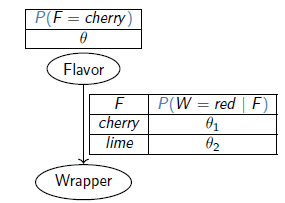
\includegraphics[width=0.2\linewidth]{images/wrapper_bn.png}
\end{figure}

the \linkterm{likelihood}{def:bayesian_terms} for cherry in green wrapper is $P(F=\text{cherry}, W=\text{green} \mid h_{\theta, \theta_1, \theta_2})$:
\[
= P(F=\text{cherry} \mid h_{\theta, \theta_1, \theta_2}) \cdot P(W=\text{green} \mid F=\text{cherry}, h_{\theta, \theta_1, \theta_2}) = \theta \cdot (1-\theta_1)
\]
}{}

When we have $\textbf{d}$ observations for $N$ candies, we count the occurrences of every single event:
\begin{itemize}
    \item $c$: total cherry candies 
    \item $\ell$: total lime candies
    \item $r_c$: total red wrapped cherry candies
    \item $g_c$: total green wrapped cherry candies \hfill ($r_c + g_c = c$)
    \item $r_{\ell}$: total red wrapped lime candies 
    \item $g_{\ell}$: total green wrapped lime candies \hfill ($r_{\ell} + g_{\ell} = \ell$)
\end{itemize}

We want to calculate $P(\mathbf{d} \mid h_{\theta, \theta_1, \theta_2})$. Let's build it systematically from a single event up to the full sequence $N$.

Every single candy drawn from the bag represents a joint assignment to two discrete \linkterm{random variables}{def:random_variable}: its Flavor ($F \in \{\text{cherry}, \text{lime}\}$) and its Wrapper color ($W \in \{\text{red}, \text{green}\}$). 

Because we have a \linkterm{Bayesian Networks}{jpd_BN}, we know that $P(F, W) = P(F)P(W \mid F)$, we compute the likelihood of a single observation falling into one of four possible atomic categories under our continuous hypothesis $h_{\theta, \theta_1, \theta_2}$:
\begin{enumerate}
    \item \textbf{Cherry flavor in a Red wrapper:}
    \[
    P(F=\text{cherry}, W=\text{red} \mid h_{\theta, \theta_1, \theta_2}) = P(F=\text{cherry}) \cdot P(W=\text{red} \mid F=\text{cherry}) = \theta \cdot \theta_1
    \]
    \item \textbf{Cherry flavor in a Green wrapper:}
    \[
    P(F=\text{cherry}, W=\text{green} \mid h_{\theta, \theta_1, \theta_2}) = P(F=\text{cherry}) \cdot P(W=\text{green} \mid F=\text{cherry}) = \theta \cdot (1-\theta_1)
    \]
    \item \textbf{Lime flavor in a Red wrapper:}
    \[
    P(F=\text{lime}, W=\text{red} \mid h_{\theta, \theta_1, \theta_2}) = P(F=\text{lime}) \cdot P(W=\text{red} \mid F=\text{lime}) = (1-\theta) \cdot \theta_2
    \]
    \item \textbf{Lime flavor in a Green wrapper:}
    \[
    P(F=\text{lime}, W=\text{green} \mid h_{\theta, \theta_1, \theta_2}) = P(F=\text{lime}) \cdot P(W=\text{green} \mid F=\text{lime}) = (1-\theta) \cdot (1-\theta_2)
    \]
\end{enumerate}

Let our dataset $\mathbf{d} = d_{1:N}$ be a specific ordered sequence of $N$ draws. Because these trials are assumed to be independent and identically distributed (\linkterm{IID}{def:iid}), the joint likelihood of the entire dataset is computed by taking the mathematical product of the probabilities of each individual trial:
\[
P(\mathbf{d} \mid h_{\theta, \theta_1, \theta_2}) = \prod_{j=1}^{N} P(d_j \mid h_{\theta, \theta_1, \theta_2})
\]
If our data sequence consisted of just three specific draws—for instance: $d_1 = (\text{cherry}, \text{red})$, $d_2 = (\text{cherry}, \text{green})$, and $d_3 = (\text{lime}, \text{red})$—the expanded product would be written as:
\[
P(\mathbf{d} \mid h_{\theta, \theta_1, \theta_2}) = (\theta \cdot \theta_1) \cdot (\theta \cdot (1-\theta_1)) \cdot ((1-\theta) \cdot \theta_2)
\]

Because multiplication is commutative ($A \cdot B = B \cdot A$), we can reorder the terms in our massive multi-element product chain. We group identical parameter factors together into distinct algebraic bins:
\[
P(\mathbf{d} \mid h_{\theta, \theta_1, \theta_2}) = (\theta \cdot \theta) \cdot (1-\theta) \cdot (\theta_1) \cdot (1-\theta_1) \cdot (\theta_2)
\]
To scale this up to $N$ observations, we count the total frequency of each specific event across our complete dataset:
\begin{itemize}
    \item The factor $\theta$ appears exactly once for every cherry candy, totaling $c$ times $\implies \theta^c$
    \item The factor $(1-\theta)$ appears exactly once for every lime candy, totaling $\ell$ times $\implies (1-\theta)^{\ell}$
    \item The factor $\theta_1$ appears exactly once for every cherry candy with a red wrapper, totaling $r_c$ times $\implies \theta_1^{r_c}$
    \item The factor $(1-\theta_1)$ appears exactly once for every cherry candy with a green wrapper, totaling $g_c$ times $\implies (1-\theta_1)^{g_c}$
    \item The factor $\theta_2$ appears exactly once for every lime candy with a red wrapper, totaling $r_{\ell}$ times $\implies \theta_2^{r_{\ell}}$
    \item The factor $(1-\theta_2)$ appears exactly once for every lime candy with a green wrapper, totaling $g_{\ell}$ times $\implies (1-\theta_2)^{g_{\ell}}$
\end{itemize}

Multiplying these aggregated exponential bins together yields our finalized data likelihood function:
\[
P(\mathbf{d} \mid h_{\theta, \theta_1, \theta_2}) = \theta^c \cdot (1-\theta)^{\ell} \cdot \theta_1^{r_c} \cdot (1-\theta_1)^{g_c} \cdot \theta_2^{r_{\ell}} \cdot (1-\theta_2)^{g_{\ell}}
\]


We maximize the \linkterm{log-likelihood}{log_likelihood} to determine our optimal parameter configurations. Applying our logarithmic identity to the joint product function breaks the formula apart into a clean, additive optimization landscape:
\begin{align*}
L(\theta, \theta_1, \theta_2) &:= \log_2 P(\mathbf{d} \mid h_{\theta, \theta_1, \theta_2}) \\
&= \log_2 \left( \theta^c \cdot (1-\theta)^{\ell} \cdot \theta_1^{r_c} \cdot (1-\theta_1)^{g_c} \cdot \theta_2^{r_{\ell}} \cdot (1-\theta_2)^{g_{\ell}} \right) \\
&= \Big[ c \log_2(\theta) + \ell \log_2(1-\theta) \Big] \\ 
&+ \Big[ r_c \log_2 (\theta_1) + g_c \log_2 (1-\theta_1) \Big] \\ 
&+ \Big[ r_{\ell} \log_2 (\theta_2) + g_{\ell} \log_2 (1-\theta_2) \Big]
\end{align*}


Because our optimization objective is now a sum of decoupled components, computing the partial derivative with respect to any single parameter treats all other additive terms as constants, which completely drop out to $0$. This allows us to maximize each parameter independently:

\begin{enumerate}
    \item \textbf{Optimizing for $\theta$:}
    We isolate the components containing $\theta$ and set the derivative to zero:
    \[
    \frac{\partial L}{\partial \theta} = \frac{c}{\theta \ln 2} - \frac{\ell}{(1-\theta)\ln 2} = 0
    \]
    Multiplying the entire expression by the non-zero constant $\ln 2$ simplifies our root-finding problem:
    \[
    \frac{c}{\theta} - \frac{\ell}{1-\theta} = 0 \implies \frac{c}{\theta} = \frac{\ell}{1-\theta}
    \]
    Cross-multiplying and grouping like terms isolates our first parameter:
    \[
    c(1-\theta) = \ell\theta \implies c - c\theta = \ell\theta \implies c = (c+\ell)\theta \implies \theta_{\text{ML}} = \frac{c}{c + \ell}
    \]

    \item \textbf{Optimizing for $\theta_1$:}
    We isolate the components containing $\theta_1$, treating all other flavor or lime-specific terms as zero:
    \[
    \frac{\partial L}{\partial \theta_1} = \frac{r_c}{\theta_1 \ln 2} - \frac{g_c}{(1-\theta_1)\ln 2} = 0
    \]
    Clearing out the common $\ln 2$ denominator yields:
    \[
    \frac{r_c}{\theta_1} - \frac{g_c}{1-\theta_1} = 0 \implies \frac{r_c}{\theta_1} = \frac{g_c}{1-\theta_1}
    \]
    Cross-multiplying and evaluating the linear algebra gives:
    \[
    r_c(1-\theta_1) = g_c\theta_1 \implies r_c - r_c\theta_1 = g_c\theta_1 \implies r_c = (r_c+g_c)\theta_1 \implies \theta_{1,\text{ML}} = \frac{r_c}{r_c + g_c}
    \]

    \item \textbf{Optimizing for $\theta_2$:}
    We isolate the components containing $\theta_2$, treating the flavor and cherry-specific terms as zero:
    \[
    \frac{\partial L}{\partial \theta_2} = \frac{r_{\ell}}{\theta_2 \ln 2} - \frac{g_{\ell}}{(1-\theta_2)\ln 2} = 0
    \]
    Clearing out the common $\ln 2$ denominator yields:
    \[
    \frac{r_{\ell}}{\theta_2} - \frac{g_{\ell}}{1-\theta_2} = 0 \implies \frac{r_{\ell}}{\theta_2} = \frac{g_{\ell}}{1-\theta_2}
    \]
    Cross-multiplying and solving for our final parameter finishes the estimation:
    \[
    r_{\ell}(1-\theta_2) = g_{\ell}\theta_2 \implies r_{\ell} - r_{\ell}\theta_2 = g_{\ell}\theta_2 \implies r_{\ell} = (r_{\ell}+g_{\ell})\theta_2 \implies \theta_{2,\text{ML}} = \frac{r_{\ell}}{r_{\ell} + g_{\ell}}
    \]
\end{enumerate}

Summary of our decoupled parameter results:
\begin{align*}
\frac{\partial L}{\partial \theta} &= 0 &&\leadsto \theta_{\text{ML}} = \frac{c}{c + \ell} \\
\frac{\partial L}{\partial \theta_1} &= 0 &&\leadsto \theta_{1,\text{ML}} = \frac{r_c}{r_c + g_c} \\
\frac{\partial L}{\partial \theta_2} &= 0 &&\leadsto \theta_{2,\text{ML}} = \frac{r_{\ell}}{r_{\ell} + g_{\ell}}
\end{align*}

Thus, our multi-parameter \linkterm{MLP learning method}{MLP_learning} tells us that the single most likely global hypothesis $h_{\theta_{\text{ML}}, \theta_{1,\text{ML}}, \theta_{2,\text{ML}}}$ is simply the one where every individual network parameter matches its own local sample proportion from the data:
\begin{itemize}
    \item The global flavor parameter $\theta_{\text{ML}}$ is simply the proportion of cherry candies out of all drawn candies.
    \item The conditional wrapper parameter $\theta_{1,\text{ML}}$ is simply the proportion of red wrappers calculated strictly within the subset of observed cherry candies.
    \item The conditional wrapper parameter $\theta_{2,\text{ML}}$ is simply the proportion of red wrappers calculated strictly within the subset of observed lime candies.
\end{itemize}


Up to this point, our continuous parameters directly defined static properties of a distribution (like a fixed coin probability or a fixed mean). However, in many core machine learning settings—such as linear regression or continuous Bayesian network nodes—the parameters of a child node's distribution are determined dynamically as a function of its parent nodes.

\anondefinition{
A continuous random variable $Y$ follows a \defemph{Linear-Gaussian Distribution} with respect to a continuous parent random variable $X$ if the outcome of $Y$ is determined by a linear function of the observed outcome $x$ plus independent  \linkterm{Gaussian}{normal_dist} noise with a fixed \linkterm{variance}{normal_dist} $\sigma^2$. 

Instead of a fixed mean $\mu$, the mean shifts dynamically based on $x$:
\[
\mu(x) = \theta_1 x + \theta_2
\]
Where $\theta_1$ represents the slope (weight) and $\theta_2$ represents the intercept (bias). The \linkterm{conditional}{def:conditional_prob} conditional \linkterm{PDF}{pdf} of $Y$ given $X=x$ is:
\[
f(y \mid X=x) = \frac{1}{\sigma \sqrt{2\pi}} e^{-\frac{1}{2}\left(\frac{y - (\theta_1 x + \theta_2)}{\sigma}\right)^2}
\]
}{linear_gaussian_def}


Assuming the noise variance $\sigma^2$ is fixed and given, our learning goal is to discover the two real-valued coefficients. Thus, our continuous hypothesis space is $\mathcal{H} = \mathbb{R} \times \mathbb{R}$.

\commandnote{
We write $\mathcal{N}(y; \theta_1 x + \theta_2, \sigma^2)$ to represent a standard \linkterm{Gaussian (Normal) distribution}{normal_dist} curve for the variable $y$, where its the mean $\mu$ is dynamically calculated using the linear equation $\theta_1 x + \theta_2$, and its spread is determined by the variance parameter $\sigma^2$.
}

The core definition of our conditional model relates the continuous input $X$ to the continuous output $Y$ via an interval-based probability statement:
\[
P(y_1 \le Y \le y_2 \mid X = x) = \int_{y_1}^{y_2} \mathcal{N}(y; \theta_1 x + \theta_2, \sigma^2) \,dy = \int_{y_1}^{y_2} \frac{1}{\sigma \sqrt{2\pi}} e^{-\frac{1}{2}\left(\frac{y - (\theta_1 x + \theta_2)}{\sigma}\right)^2} \,dy
\]

\begin{figure}[H]
    \centering
    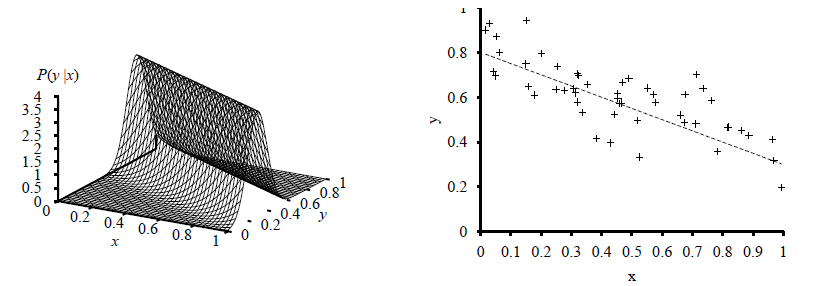
\includegraphics[width=0.5\linewidth]{images/linear_gaussian.png}
\end{figure}

\begin{itemize}
    \item \textbf{The 3D Probability Surface (Left Graph):} This plot displays the conditional probability density $P(y \mid x)$ as a continuous surface. Notice that if you freeze $x$ at any single constant slice, the cross-section along the $y$-axis forms a perfect, symmetric Gaussian bell curve. As $x$ increases, the peak of this bell curve moves smoothly along a straight linear track, while the width ($\sigma$) of the curve stays perfectly constant.
    \item \textbf{The 2D Scatter Plot (Right Graph):} This plot shows a collection of discrete data observations alongside the estimated linear regression line $y = \theta_1 x + \theta_2$. The line represents the expected value (the moving mean $\mu(x)$) for any input $x$. The actual data points do not land perfectly on the line; instead, they are scattered above and below it. This vertical dispersion is the visual manifestation of the Gaussian noise, where points cluster densely near the line and grow sparser farther away.
\end{itemize}

When we transition from describing the model's theoretical properties to actually performing parameter estimation using a collected training dataset, our perspective shifts from calculating integration areas to evaluating density heights.

Our training dataset $\mathbf{d} = \{(x_1, y_1), (x_2, y_2), \dots, (x_N, y_N)\}$ does not arrive in the form of broad spatial intervals $[y_1, y_2]$. Instead, we are given $N$ exact, singular point coordinates observed from our system. 

To determine how well a particular candidate hypothesis $h_{\theta_1, \theta_2}$ explains these precise observations, we evaluate the \textbf{likelihood density profile} at those exact coordinate pairs. This means we take our fixed coordinate values $x_i$ and $y_i$ and calculate the vertical height of the conditional PDF directly:
\[
f(y_i \mid X = x_i) = \frac{1}{\sigma \sqrt{2\pi}} e^{-\frac{1}{2}\left(\frac{y_i - (\theta_1 x_i + \theta_2)}{\sigma}\right)^2}
\]

Because our parameter optimization task is focused entirely on maximizing these point-wise vertical density heights across our \linkterm{IID}{def:iid} dataset, our conditional likelihood function is built directly from the product of these individual PDF outputs, bypassing the interval integration step entirely:
\[
P(\mathbf{d} \mid h_{\theta_1, \theta_2}) = \prod_{i=1}^{N} \frac{1}{\sigma \sqrt{2\pi}} e^{-\frac{1}{2}\left(\frac{y_i - (\theta_1 x_i + \theta_2)}{\sigma}\right)^2} = \prod_{i=1}^{N} \frac{1}{\sqrt{2\pi}\sigma} e^{-\frac{(y_i - (\theta_1 x_i + \theta_2))^2}{2\sigma^2}}
\]
Our objective is to maximize this product with respect to our target parameters $\theta_1$ and $\theta_2$.


To find the analytical maximum safely without encountering numerical underflow, we pass this product through our \linkterm{log-likelihood}{log_likelihood}
\[
L(\theta_1, \theta_2) = \ln P(\mathbf{d} \mid h_{\theta_1, \theta_2}) = \sum_{i=1}^{N} \ln \left( \frac{1}{\sqrt{2\pi}\sigma} e^{-\frac{(y_i - (\theta_1 x_i + \theta_2))^2}{2\sigma^2}} \right)
\]

Using logarithmic expansion identities ($\ln(A \cdot B) = \ln A + \ln B$ and $\ln(e^Z) = Z$), we pull the exponent down and isolate the terms:
\[
L(\theta_1, \theta_2) = \sum_{i=1}^{N} \left( \ln\left(\frac{1}{\sqrt{2\pi}\sigma}\right) - \frac{(y_i - (\theta_1 x_i + \theta_2))^2}{2\sigma^2} \right)
\]
Distributing the summation across both independent parts yields:
\[
L(\theta_1, \theta_2) = N \ln\left(\frac{1}{\sqrt{2\pi}\sigma}\right) - \frac{1}{2\sigma^2} \sum_{i=1}^{N} \left(y_i - (\theta_1 x_i + \theta_2)\right)^2
\]

To optimize this function with respect to $\theta_1$ and $\theta_2$, we evaluate how the components behave:
\begin{enumerate}
    \item The leading term, $N \ln\left(\frac{1}{\sqrt{2\pi}\sigma}\right)$, is a fixed constant that depends strictly on the sample size and the pre-determined noise parameter $\sigma$. Because it contains no dependency on our optimization variables $\theta_1$ or $\theta_2$, it has a derivative of zero and can be dropped from the maximization argmax.
    \item Multiplying our remaining function by the positive scalar constant $\frac{1}{2\sigma^2}$ scales the output but leaves the horizontal location of the optimal peak untouched. 
    \item Finally, maximizing a function with a negative sign ($-$) is mathematically identical to minimizing its positive counterpart. 
\end{enumerate}

Therefore, inverting the sign allows us to transform the maximum likelihood density problem into a clean minimization task:
\[
\arg\max_{\theta_1, \theta_2} L(\theta_1, \theta_2) = \arg\min_{\theta_1, \theta_2} \sum_{i=1}^{N} \left(y_i - (\theta_1 x_i + \theta_2)\right)^2
\]

Our derivation proves that for a Linear-Gaussian model, utilizing the log-likelihood function to find the maximum likelihood parameters is mathematically equivalent to minimizing the \textbf{sum of squared errors}:
\[
\theta_{\text{ML}} = \arg\min_{\theta_1, \theta_2} \sum_{i=1}^{N} \left(y_i - (\theta_1 x_i + \theta_2)\right)^2
\]
This reveals a key conceptual link: optimizing parameters to maximize the statistical likelihood under Gaussian noise yields the exact same solution as the purely geometric framework of Ordinary Least Squares (OLS) linear regression.
